% 113-78(113쪽) — x>=0 에서 y=F(x) 의 그래프(원점에서 출발해 x=b 에서 극대, c 에서 x 축을 지나 x=d 에서 극소, e 에서 다시 x 축을 지남). 스캔 화질이 낮아 TikZ 로 다시 그림.
% 원문에 있는 것만: x 축 위 라벨 a, b(아래)·c, d, e(위) · x=a, x=b 의 위쪽 안내 파선과 x=d 의 아래쪽 안내 파선 · 라벨 O, x, y, y=F(x).
% 눈금 숫자·좌표값은 원문에 없으므로 넣지 않는다(보기의 참·거짓이 그림에서 수치로 읽히지 않게).
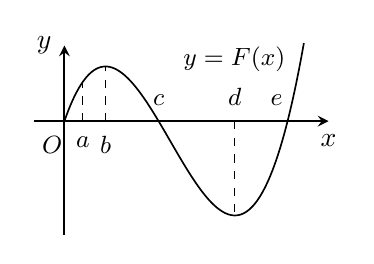
\begin{tikzpicture}[x=0.52cm, y=0.40cm, line width=0.5pt]
  \draw[->, >=stealth, line width=0.7pt] (-0.75,0) -- (6.45,0) node[below=1pt] {$x$};
  \draw[->, >=stealth, line width=0.7pt] (0,-3.6) -- (0,2.4) node[left=1pt] {$y$};
  \node[below=2pt, font=\small] at (-0.3,0) {$\pt{O}$};
  % 좌표 안내 파선(원문)
  \draw[dashed, line width=0.35pt] (0.45,0) -- (0.45,1.249);
  \draw[dashed, line width=0.35pt] (1.004,0) -- (1.004,1.735);
  \draw[dashed, line width=0.35pt] (4.163,0) -- (4.163,-2.992);
  % 그래프 — 원점에서 출발해 c, e 에서 x 축을 지나는 모양(원문 그대로)
  \draw[line width=0.6pt, domain=0:5.85, samples=200, smooth] plot (\x, {0.3*\x*(\x-2.3)*(\x-5.45)});
  \node[below=2pt, font=\small] at (0.45,0) {$a$};
  \node[below=2pt, font=\small] at (1.004,0) {$b$};
  \node[above=2pt, font=\small] at (2.3,0) {$c$};
  \node[above=2pt, font=\small] at (4.163,0) {$d$};
  \node[above=2pt, font=\small] at (5.18,0) {$e$};
  \node[font=\small] at (4.15,1.95) {$y=F(x)$};
\end{tikzpicture}
